\chapter{Week 1: Methods and Organelles}\label{Week 1: Methods and Organelles}
% chktex-file 1
% chktex-file 8
% chktex-file 27

\section{Background}\label{Background}
\begin{itemize}
  \item \jjj{Describe the steps in tissue preparation for microscopy:}
    \begin{itemize}
      \item \jjj{Fixation}: typically the first step in the preparation of histological sections in where tissues samples are treated with fixatives as a means to preserve and protect from biological decay.
        \begin{itemize}
          \item \jjj{Fixatives}: solutions, compounds, or others means meant to either disable degradative enzymes, induce cross-linking (stabilizing proteins), or protect from extrinsic damage.
        \end{itemize}
      \item \jjj{Embedding}: the process of placing tissues in a harder medium (e.g., paraffin and plastic resins) as a means to allow for thin slicing of tissue.
        \begin{itemize}
          \item Embedding occurs later in the process of preparation; once a tissue is fixed it must first undergo a series of steps:
          \begin{itemize}
            \item \jjj{Dehydration}: the removal of water using ethanol.
            \item \jjj{Clearing}: replacement of an organic solvent miscible with both alcohol and the embedding medium, giving a translucent appearance.
            \item \jjj{Infiltration}: evaporation of the clearing solvent via exposure to heat (50--\SI{60}{\celsius}) promoting the final embedding of tissue into the medium.
          \end{itemize}
        \end{itemize}
      \item \jjj{Staining}: used as a means to increase contrast in tissue or specific features of tissue that are of interest as most biology tissue has very little inherent contrast.
        \begin{itemize}
          \item \bbb{Basophilic}: dyes that have an affinity for \bbb{anionic} (net \bbb{negative} charge) cells parts.
            \begin{itemize}
              \item E.g., hematoxylin, toluidine blue, alcian blue, and methylene blue.
            \end{itemize}
          \item \rrr{Acidophilic}: dyes that have an affinity for \rrr{cationic} (net \rrr{positive} charge) cell parts.
            \begin{itemize}
              \item E.g., eosin, orange G, and acid fuchsin
            \end{itemize}
        \end{itemize}
    \end{itemize}
  \item \jjj{What does H \& E Stain?}
    \begin{itemize}
      \item \chap{Hematoxylin (H)} and \amp{eonsin (E)} stains are among the most commonly used stains. 
        \begin{itemize}
          \item As mentioned above, hematoxylin acts as a \bbb{basophilic dye}, turning negatively charge organelles like the cell nucleus, RNA-rich regions of cytoplasm, cartilage, anywhere from \bbb{blue} \chap{\to} \xxx{purple}.
          \item Eosin acts as an \rrr{Acidophilic dye}, typically turning \amp{cationic structures pink}; sometimes it is considered to be a \jjj{counterstain}, i.e., typically a secondary dye that is meant to distinguish features.
        \end{itemize}
    \end{itemize}
  \item \jjj{What does PAS Stain?}
    \begin{itemize}
      \item \xxx{Periodic acid-Schiff (PAS)} utilizes hexose rings of polysaccharides and other carbohydrate rich structures to stain macromolecules \xxx{purple} \to~\fff{magenta}.
    \end{itemize}
  \item \jjj{Describe Enzyme Histochemistry.}
    \begin{itemize}
      \item Enzyme histochemistry is a method for localizing cellular structures using specific enzymatic activity in such structures.
      \item Preservation of enzymes often requires non-fixed or mildly fixed tissue and generally adhere to the following steps:
        \begin{enumerate}
          \item Tissues sections are immersed in solution containing the substrate of the enzyme to be localized.
          \item The enzyme is exposed to and allowed to act on the substrate.
          \item A marker compound is introduced and reacted with the product from step 2.
          \item Location is determined via precipitation of the insoluble product, which must be visible a light or electron microscopy, over the site of the enzyme.
        \end{enumerate}
      \item Phosphatase, dehydrogenase, and peroxidase are common examples of enzymes detected with histochemistry.
    \end{itemize}
  \item \jjj{How does Immunohistochemistry work?}
    \begin{itemize}
      \item Immunohistochemistry (IHC): the use of labeled antibodies and antigens to identify and localize many proteins and macromolecules that lack specific enzymatic activity. 
      \item Visualization of such interactions are commonly  accomplished with either:
        \begin{itemize}
          \item Chromogenic immunohistochemistry (CIH): use of antibodies conjugated to an enzyme that catalyzes a color-producing reaction.
          \item Immunofluorescence: tagging of a fluorophore (fluorescein, rhodamine) to an antibody. 
        \end{itemize}
      \item Common used in diagnosis of abnormal cells such as those in cancerous tumors. 
    \end{itemize}
\end{itemize}

\section{Microscopic Techniques}
\begin{itemize}
  \item \jjj{Bright field}: a very common method that uses ordinary light and stained structures to discern differences and cell structures. 
  \begin{center}
    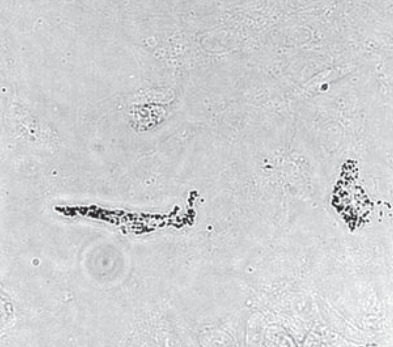
\includegraphics[scale=0.45]{images/week-1-1a.jpg}
  \end{center}
  \item \jjj{Phase contrast}: uses differences in refractive index of natural cell and tissue components; allows for observation of living cells.
  \begin{center}
    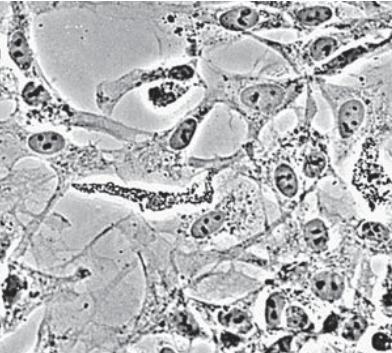
\includegraphics[scale=0.45]{images/week-1-1b.jpg}
  \end{center}
  \item \jjj{Confocal}: use of scans at successive focal planes with a more focused light beam, usually from a laser, to construct a 3D image.
  \begin{center}
    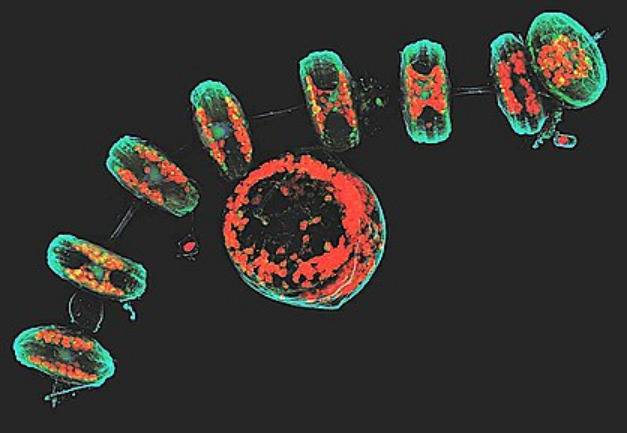
\includegraphics[scale=0.50]{images/week-1-1c.jpg}
  \end{center}
  \item \jjj{Fluorescent}: use of longer wavelengths emitted via specific perturbations of cellar substances using a specific wavelength (usually UV). Useful for identification of cells and components that have affinity for specific fluorescent compounds. 
  \begin{center}
    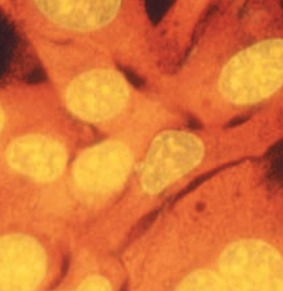
\includegraphics[scale=0.60]{images/week-1-1d.jpg}
    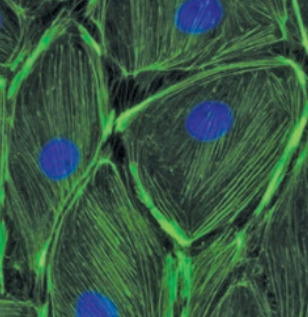
\includegraphics[scale=0.55]{images/week-1-1e.jpg}
  \end{center}
  \newpage
  \item \jjj{Transmission Electron Microscopy (TEM)}: a high resolution (3 nm) that allows for particles to be magnified many times via transmission of electrons though a specimen; very thin tissue sections are used and a flat image is made from the intersection of the electron beam and the sample.
  \begin{center}
    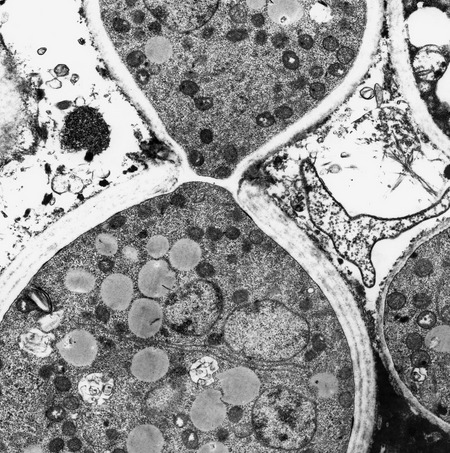
\includegraphics[scale=0.60]{images/week-1-1g.jpg}
  \end{center}
  \item \jjj{Scanning Electron Microscopy (SEM)}: used to provide a high resolution view of the surface of cells, tissues, and organs. Unlike TEM, SEM does not intersect with the specimen, instead the electrons are reflected by a coating and then collected, analyzed, and used to generate a 3D view.
  \begin{center}
    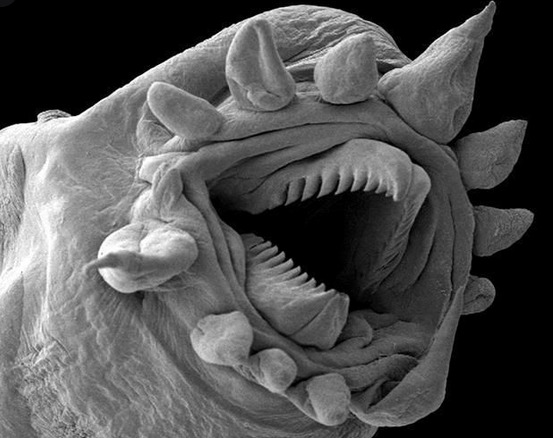
\includegraphics[scale=0.60]{images/week-1-1f.jpg}
  \end{center}
\end{itemize}
\clearpage
\section{Organelles and Cytoplasmic Inclusions}
\begin{multicols}{2}
\begin{itemize}
  \item \jjj{Nucleus}: a large membrane bound organelle that contains chromatin, the nucleolus, and nucleoplasm. \\ 
  \textit{Size}: \emph{5--20 \si{\micro m}}, the largest organelle. \\
  \begin{center}
    \hspace{-30pt}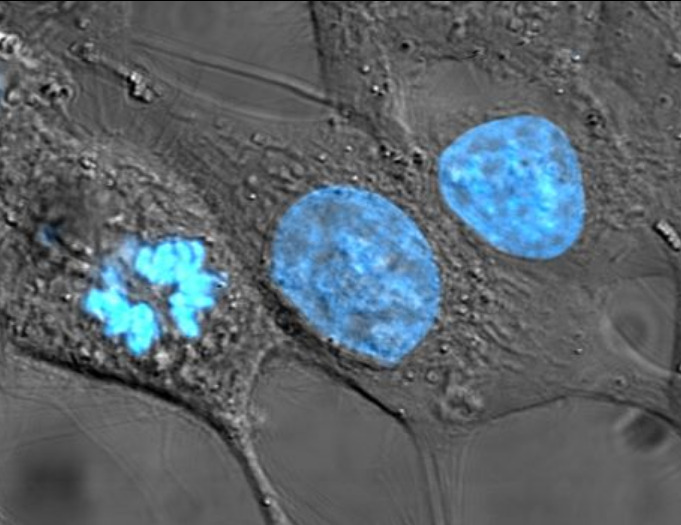
\includegraphics[width=0.65\columnwidth]{images/week-1-nucleus.jpg}
  \end{center}
  \item \jjj{Nucleolus}: large, dense structure within the nucleus that functions in the synthesis of ribosomes. \\
  \textit{Size}: \emph{0.5--5 \si{\micro m}}, smaller than nucleus.
  \begin{center}
    \hspace{-30pt}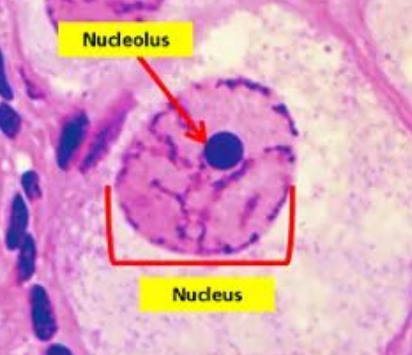
\includegraphics[width=0.65\columnwidth]{images/week-1-nucleolus.jpg}
  \end{center}
  \item \jjj{Plasma Membrane}: phospholipid bilayer containing various elements, acts as a physical barrier to regulate internal environment; maintains charge and functions in cell communication. \\
  \textit{Size}: \emph{5--10 \si{nm}}, very thin---3 orders of magnitude less than width of nucleus.
  \begin{center}
    \hspace{-30pt}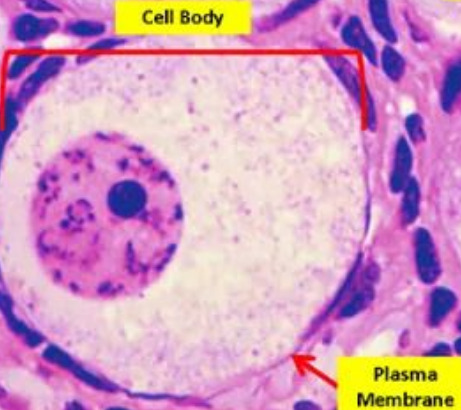
\includegraphics[width=0.65\columnwidth]{images/week-1-plasma.jpg}
  \end{center}
  \item \jjj{Rough ER}: interconnect membrane that modifies, transports, and stores proteins produced by attached ribosomes. \\
  \textit{Size}: \emph{5--8 \si{nm} thick, \emph{20-30 \si{nm} wide}}, membrane of rER thin, while the lumen is wide and surrounds nucleus (often).
  \begin{center}
    \hspace{-30pt}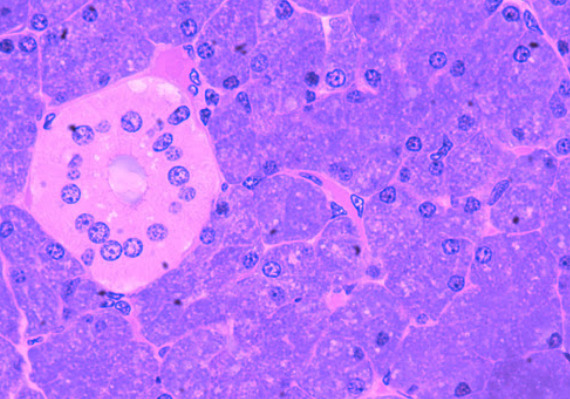
\includegraphics[width=0.65\columnwidth]{images/week-1-rer.jpg}
  \end{center}
  \item \jjj{Smooth ER}: Like rER, but lacking ribosomes; synthesizes, transports, and stores lipids; metabolizes carbohydrates, toxins (of various types); and forms vesicles and peroxisomes.\\
  \textit{Size}: lumen is \emph{30--60 \si{nm}} thick, larger than rER\@; overall fraction of cell varies.
  \begin{center}
    \hspace{-30pt}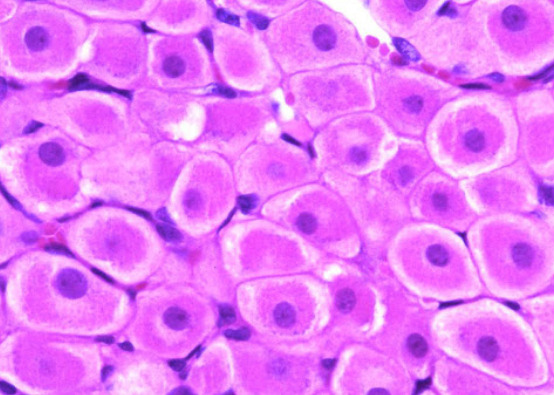
\includegraphics[width=0.65\columnwidth]{images/week-1-ser.jpg}
  \end{center}
  \item \jjj{Golgi Apparatus}: modifies, packages, and sorts materials that arrive from the ER\@; forms secretory vesicles/lysosomes. \\
  \textit{Size}: \emph{2--5 \si{mm}}, stacks of flat membranes, can occupy large portion of cell.
  \begin{center}
    \hspace{-30pt}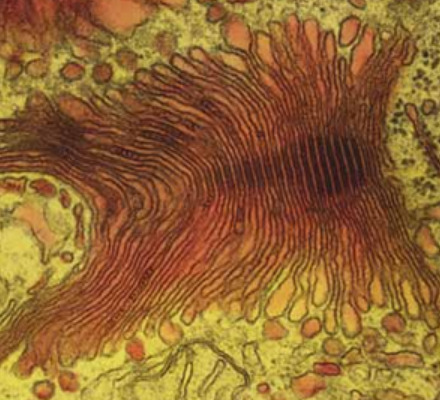
\includegraphics[width=0.6\columnwidth]{images/week-1-golgi.jpg}
  \end{center}
  \item \jjj{Vesicles}: transports cellular material \\
  \textit{Size}: \emph{30--100 \si{nm}}, large range varies among different types of vesicles, still relatively small.
  \begin{center}
    \hspace{-30pt}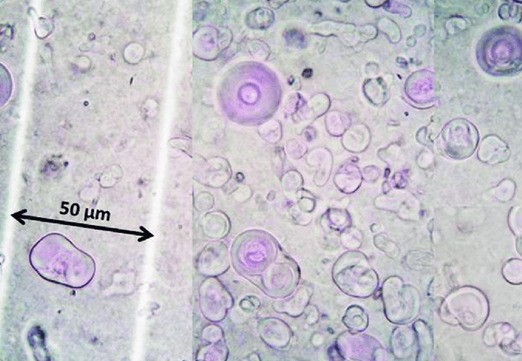
\includegraphics[width=0.75\columnwidth]{images/week-1-vesicle.jpg}
  \end{center}
  \item \jjj{Mitochondria}: \small{\textit{the powerhouse of the cell}}. \\
  \textit{Size}: \emph{0.5--1 \si{\micro m}}, decently sized, but still smaller than other organelles in the cell.
  \begin{center}
    \hspace{-30pt}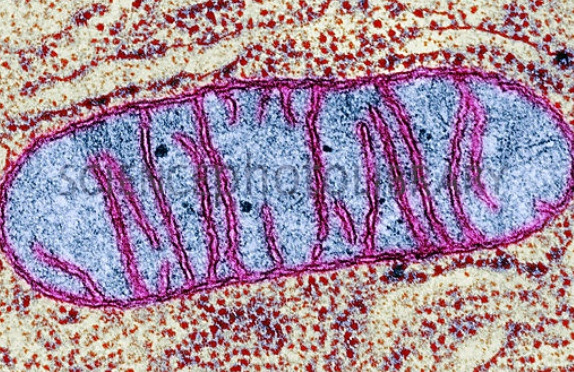
\includegraphics[width=0.75\columnwidth]{images/week-1-powerhouse.jpg}
  \end{center}
  \item \jjj{Endosomes}: collection of intracellular sorting organelles, originating from trans Golgi network that move molecules and ligands to lysosomes (L), or recycled back to cell membrane.\\
  \textit{Size}: \emph{1--50 \si{\micro m}}, depends on stage;\\
  (E)rly forms dynamic tubular network, can be long. % chktex 36
  (M)vbs (late) lack tubes.\\ % chktex 36
  TEM, not light microscope below*
  \begin{center}
    \hspace{-30pt}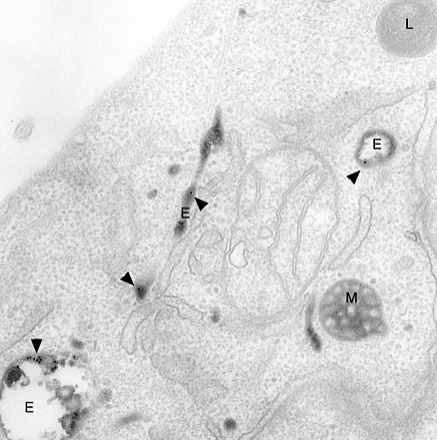
\includegraphics[width=0.75\columnwidth]{images/week-1-endosome.jpg}
  \end{center}
  \item \jjj{Lysosomes}: spherical-shaped from Golgi, contains digestive enzymes to break down microbes and materials.\\
  \textit{Size}: \emph{0.5--1 \si{\micro m}}, rather small, TEM used below instead of light microscope.
  \begin{center}
    \hspace{-30pt}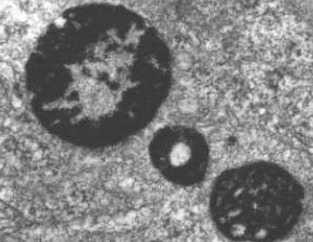
\includegraphics[width=0.69\columnwidth]{images/week-1-lysosome.jpg}
  \end{center}
  \item \jjj{Peroxisomes}: formed via ER or fission; contains enzymes to break down specific harmful substances, also used for beta oxidation of fatty acids. \\
  \textit{Size}: \emph{0.1--1 \si{\micro m}}, typically smaller than lysosomes, can be similar sized.
  \begin{center}
    \hspace{-30pt}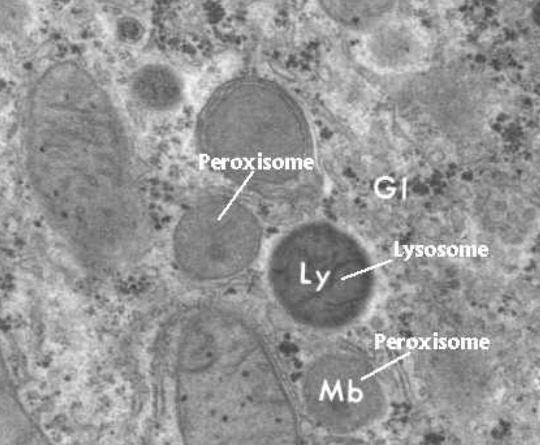
\includegraphics[width=0.69\columnwidth]{images/week-1-peroxisome.jpg}
  \end{center}
  \item \jjj{Cytoskeleton}: organized network of \{actin, micro-, intermediate\} filaments, and microtubules and other proteins.\\
  \textit{Size}: \emph{7 \si{nm}}, varies, depending on structure and filaments used.
  \begin{center}
    \hspace{-30pt}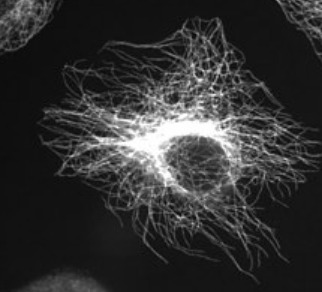
\includegraphics[width=0.69\columnwidth]{images/week-1-cytoskeleton.jpg}
  \end{center}
  \item \jjj{Ribosomes}: composed of protein and rRNA and engage in protein synthesis; can be on rER, in plasma membrane, in lysosomes, and free in cell. \\
  \textit{Size}: \emph{20--30 \si{nm}}, varies, organized into both large and small subunits.
  \begin{center}
    \hspace{-30pt}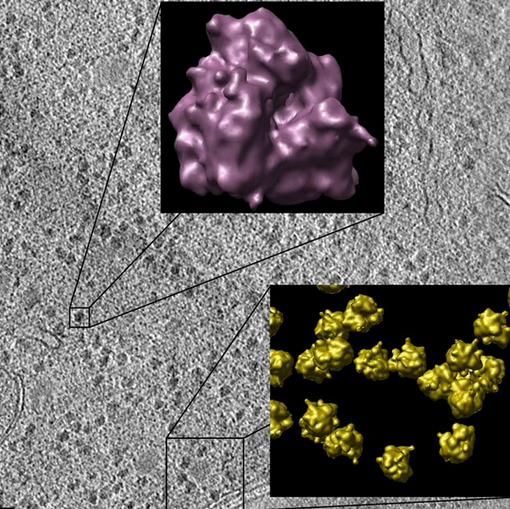
\includegraphics[width=0.8\columnwidth]{images/week-1-ribosome.jpg}
  \end{center}
  \item \jjj{Glycogen granules}: aggregates of carbohydrate polymer in which glucose is stored, notably in liver cells\\
  \textit{Size}: \emph{20--30 \si{\micro m}}, many can cluster.
  \begin{center}
    \hspace{-30pt}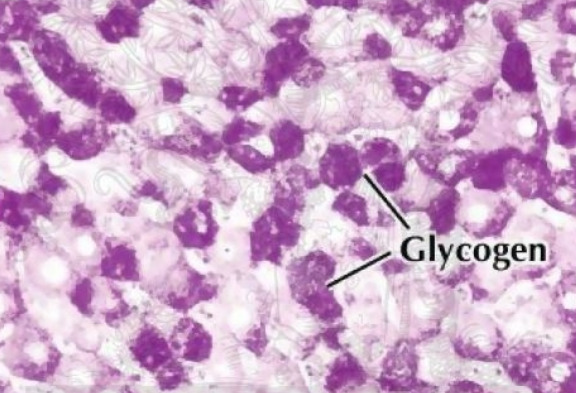
\includegraphics[width=0.8\columnwidth]{images/week-1-glycogen.jpg}
  \end{center}
  \item \jjj{Lipid droplets}: accumulations of lipid-filling adipocytes. \\
  \textit{Size}: \emph{20--40 \si{nm} to 100 \si{\micro m}}, can be removed, can take up majority of cell.
  \begin{center}
    \hspace{-30pt}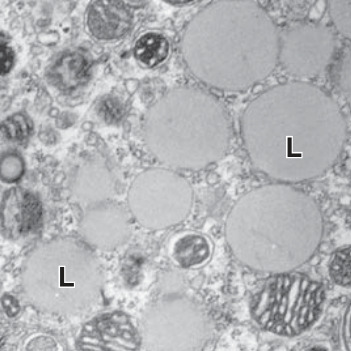
\includegraphics[width=0.7\columnwidth]{images/week-1-liquid.jpg}
  \end{center}
  \end{itemize}
\end{multicols}
  \subsection{Labeled Diagram of a Eukaryotic Cell}
  \begin{figure*}[h]
    \centering
    \def\svgwidth{\textwidth}
    \input{images/animal-cell.pdf_tex}
  \end{figure*}

  
\clearpage
\section{Mitotic Phases}
\begin{center}
  \chemname{\Image{3.5cm}{images/week-1-mp1.jpg}}{\jjj{Interphase}}\Arrow
  \chemname{\Image{3.5cm}{images/week-1-mp2.jpg}}{\jjj{Prophase}}\Arrow
  \chemname{\Image{3.5cm}{images/week-1-mp3.jpg}}{\jjj{Prometaphase}}
\end{center}
\begin{center}
  \chemname{\Image{3.5cm}{images/week-1-mp4.jpg}}{\jjj{Metaphase}}\Arrow
  \chemname{\Image{3.5cm}{images/week-1-mp5.jpg}}{\jjj{Anaphase}}\Arrow
  \chemname{\Image{3.5cm}{images/week-1-mp6.jpg}}{\jjj{Telophase}}
\end{center}

\begin{center}
  \def\svgwidth{0.95\textwidth}
    \input{images/cell-cycle-2.pdf_tex}
  \def\svgwidth{0.6\textwidth}
    \input{images/cell-cycle.pdf_tex}
\end{center}

\begin{itemize}
  \item \emph{\textbf{Interphase}}: The long period between mitosis (the \tsec{G\(_1\)}, \rrr{S}, and \igg{G\(_2\)} phases) that takes place before division is able to occur again.
  \item The \xxx{\textbf{mitotic phase}} consists of: 
    \begin{itemize}
      \item \jjj{Prophase \(\pm 1\) \normalfont{hr}}: the first stage where the nucleolus disappears, replicated chromatin condenses and each sister chromatid joins with the centromere. 
      \item \jjj{Prometaphase}: not always presented as a distinct section from prophase, instead it meant to describe processes typically found in \tsec{later parts of prophase}---i.e., where nuclear lamina and pore complexes disperse in cytoplasmic membrane vesicles---and \tsec{early parts of metaphase}---i.e., the attachment to kinetochores, which help with alignment, and other processes.
      \item \jjj{Metaphase \(< 1\) \normalfont{hr}}: further condensation of chromosomes, the cell is more spherical, and microtubules move the chromosomes towards the equatorial plate.
      \item \jjj{Anaphase \(\leq \tfrac{1}{2}\) \normalfont{hr}}: the chromosomes separate towards opposite spindle poles and reach maximum condensation.
      \item \jjj{Telophase \normalfont{(minutes)}}: the final stage, where effects of prophase and prometaphase are reversed, and a contractile ring of actin filament forms to allow for constriction and thus cytokinesis to occur.
    \end{itemize}
\end{itemize}

\newpage
\section{Apoptosis Events}\label{Apoptosis Events}
\begin{itemize}
  \item \jjj{DNA fragmentation}: endonucleases are activated, cleaving DNA into fragments. 
  \begin{center}
    \Image{4.2cm}{images/week-1-apf1.jpg}\Arrow
    \Image{4.2cm}{images/week-1-apf2.jpg}
  \end{center}
  \item \jjj{Decrease of cell volume}: destruction of the cytoskeleton and chromatin causing dense (dark purple stained) pyknotic nuclei. 
  \begin{center}
    \Image{4.2cm}{images/week-1-apf2.jpg}\Arrow
    \Image{4.2cm}{images/week-1-apf3.jpg}
  \end{center}
  \item \jjj{Membrane blebbing}: shrinking of the cell causes the plasma membrane to undergo dramatic shape changes, producing ``blebbing'' structures as proteins are degraded and lipid mobility increases.
  \begin{center}
    \Image{4cm}{images/week-1-apf4.jpg}\Arrow
    \Image{4cm}{images/week-1-apf5.jpg}\Arrow
    \Image{4cm}{images/week-1-apf6.jpg}
  \end{center}
  \item \jjj{Formation of apoptotic bodies (and phagocytic removal)}: membrane-bound remnants of cytoplasm and nucleus into even smaller fragments, forming apoptotic bodies. Phospholipids on these bodies induce the phagocytosis by neighboring cells (or white blood cells).
  \begin{center}
    \Image{4.2cm}{images/week-1-apf7.jpg}\Arrow
    \Image{4.2cm}{images/week-1-apf8.jpg}
  \end{center}
\end{itemize}

\newpage
\section{Ross and Paulina Atlas Plates}\label{Ross and Paulina Atlas Plates}
\begin{itemize}
  \item \jjj{Stratified squamous epithelium (plate 2)}: deeper cells, especially those in the basal layer, are small with little cytoplasm making the nuclei appear closely packed.
    \begin{itemize}
      \item Larger cells flatten out and form disc-like squames (squamous; square-flat).
      \item The deeper cells may be columnar or cuboidal.
      \item No intracellular space and flexibility around size allows for constant abrasion; useful for mouth, esophagus, and vagina. 
    \end{itemize}
  \begin{center}
    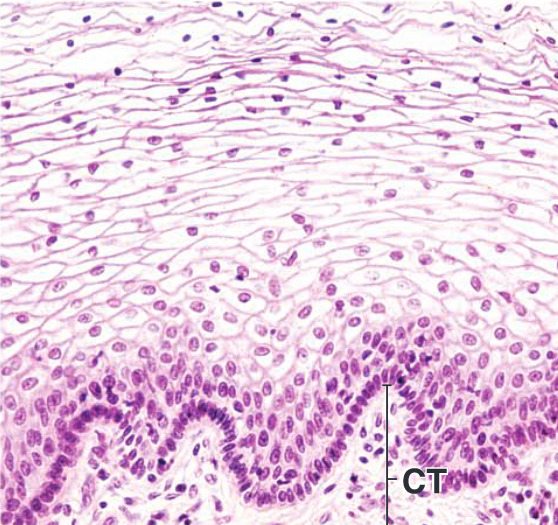
\includegraphics[scale=0.375]{images/week-1-rp1.jpg}
    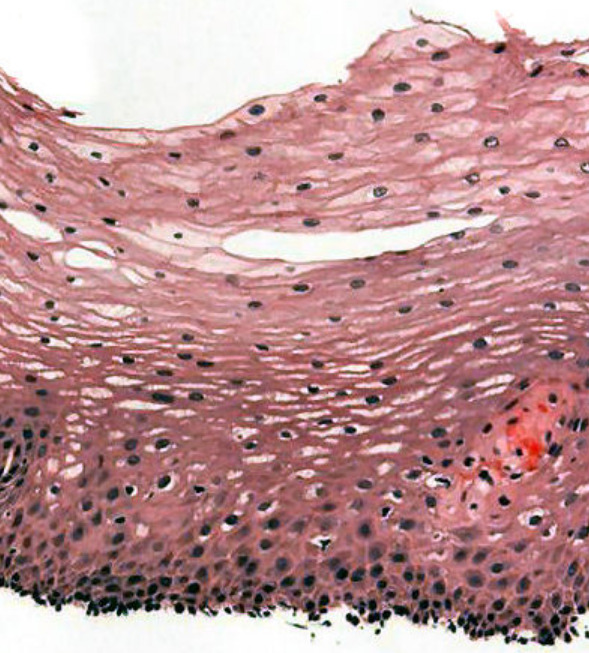
\includegraphics[scale=0.302]{images/week-1-rp2.jpg}
  \end{center}
  \item \jjj{Simple cuboidal epithelium (plate 2)}: a single layer of flax of cuboidal (cube-like) cells, with large spherical central nuclei.
    \begin{itemize}
      \item Being on the surface layer allows cells perform secretion and absorption.
      \item Found on surface of ovaries, lining of nephrons, walls of renal tubules, and parts of the eye, thyroid, and salivary glands.
    \end{itemize}
  \begin{center}
    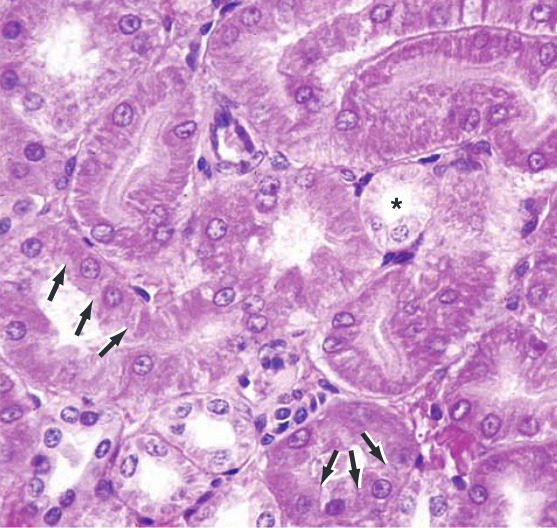
\includegraphics[scale=0.38]{images/week-1-rp3.jpg}
    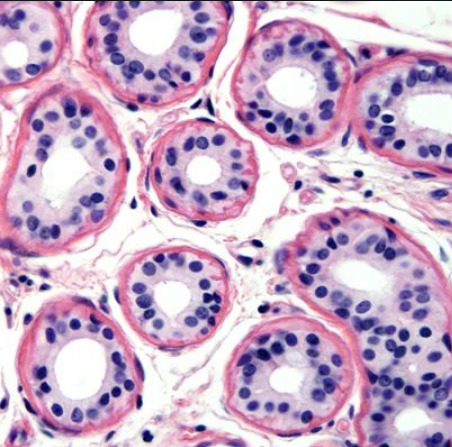
\includegraphics[scale=0.45]{images/week-1-rp4.jpg}
  \end{center}
  \newpage
  \item \jjj{Skeletal muscle (plate 22)}: one of the three major muscle types that forms striated muscle tissue and generally under control of the somatic nervous system. 
    \begin{itemize}
      \item Below is a cross-section (left) of a muscle fascicle and a longitudinal-section (right) of a gluteraldehyde. 
      \item Muscle fibers (MF) exhibit polygonal shape and vary only slightly in width. 
      \item Muscle fiber nuclei (MFN) are embedded within the extreme periphery of the fiber.
      \item Fibroblast nuclei (FN) lie outside the muscle fiber; they both smaller and more dense than the MFN\@.
      \item Capillaries (C) are present between the muscle fibers.
    \end{itemize}
  \begin{center}
    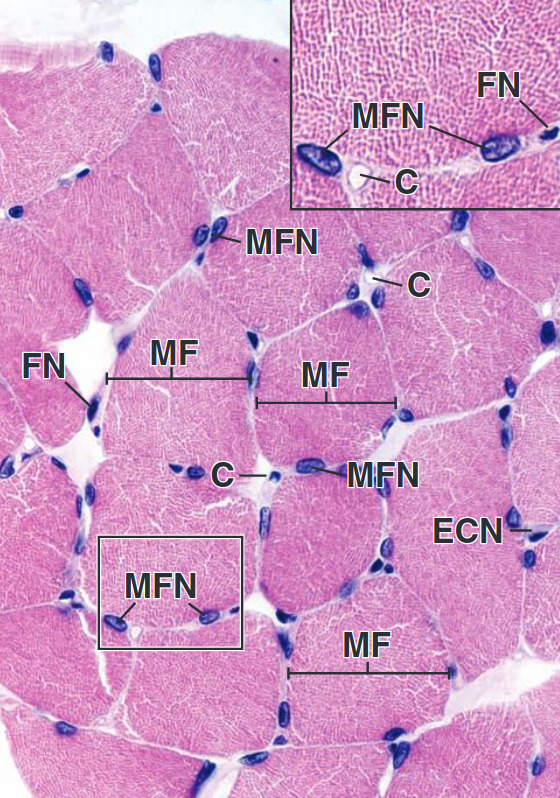
\includegraphics[scale=0.25]{images/week-1-rp5.jpg}
    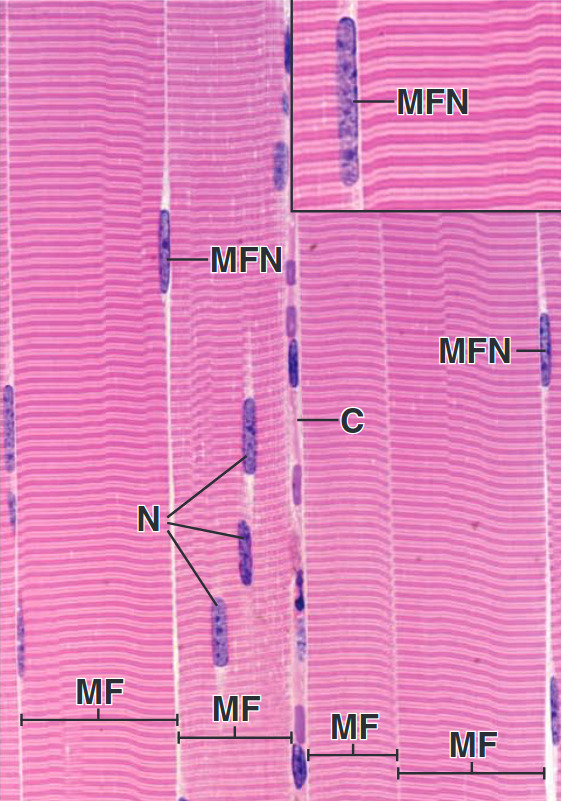
\includegraphics[scale=0.25]{images/week-1-rp6.jpg}
  \end{center}
  \item \jjj{Cardiac muscle (plate 24)}: another major muscle type that constitutes that main tissues of the walls of the heart; it is involuntary, striated muscle. 
    \begin{itemize}
      \item Below are a longitudinal-section (1) and cross-sections (2), each with an increased resolution respectively. 
      \item Intercalated discs (ID) very pronounced cross-bands, if they are stained for; they oppose cell-to-cell contacts which promotes end-to-end alignment of cells.
      \item Connective tissue cells (CT): surrounds bundles of fibers, and more delicate CT surrounds individual MF\@.
    \end{itemize}
  \begin{center}
    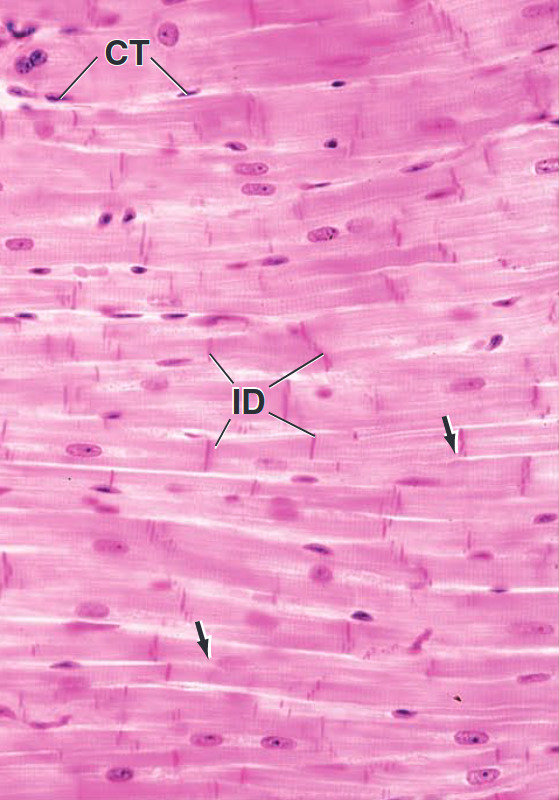
\includegraphics[scale=0.18]{images/week-1-rp7.jpg}
    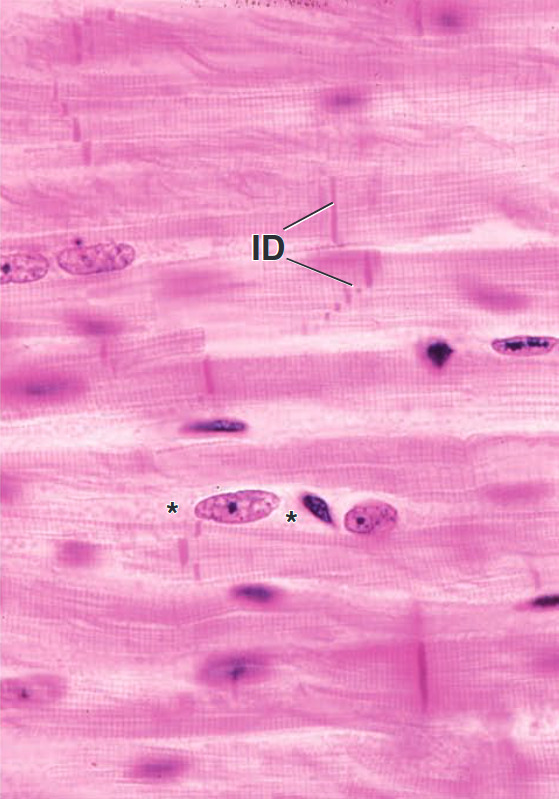
\includegraphics[scale=0.18]{images/week-1-rp8.jpg}
    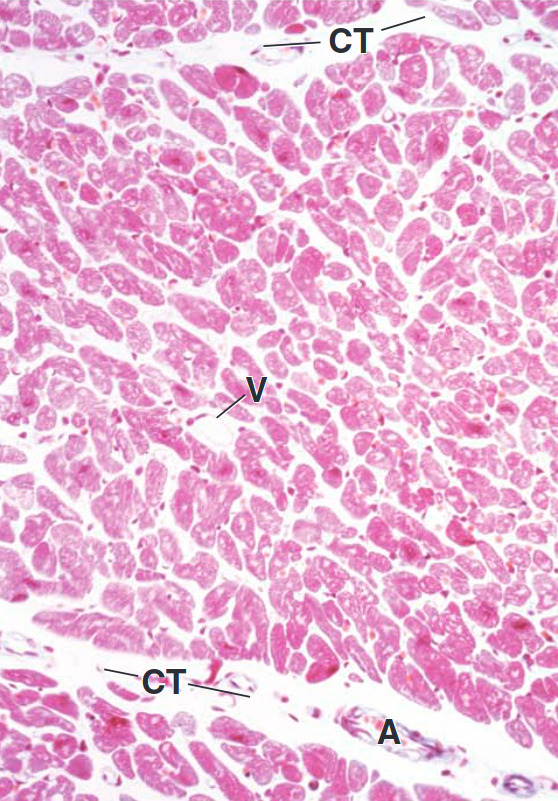
\includegraphics[scale=0.18]{images/week-1-rp9.jpg}
    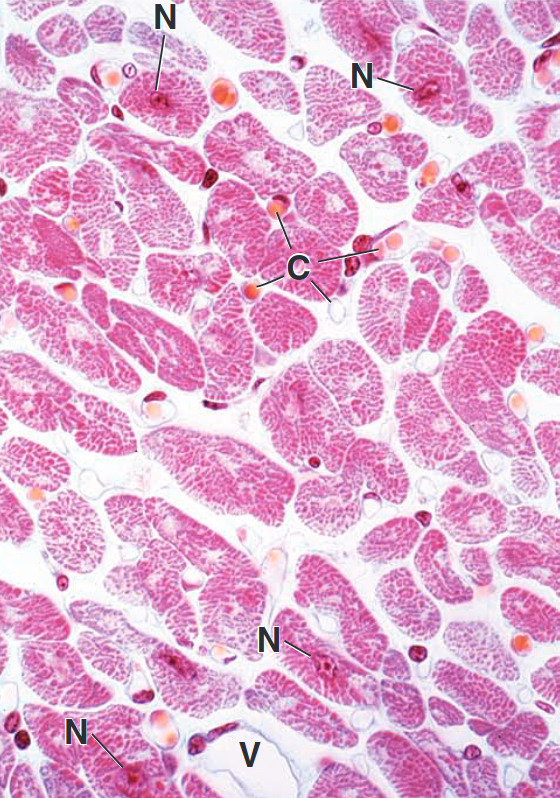
\includegraphics[scale=0.18]{images/week-1-rp10.jpg}
  \end{center}
  \item \jjj{Smooth muscle (plate 26)}: the last of the major muscle types; it is non-striated, divided into two subgroups (unitary and multi-unitary). 
    \begin{itemize}
      \item Found in hallow organs such as the stomach, intestines, urinary bladder, and uterus. Also found in passageways such as in arteries and veins, as well as tracts in the respiratory, urinary and reproductive system. 
      \item In the eye its found as ciliary muscle, a specific type of smooth muscle that dilates and contracts the iris. 
      \item Smooth muscle (SM) in the skin also helps hair stain erect.
      \item Below are cross-sectional bundles (CS) as well as longitudinally sections bundles (LS). 
      \item Dense connective tissue (DCT) separates the smooth muscle bundles, while dense irregular connective tissue (DICT) help bundle smooth muscle into circular profiles.
      \item High resolution shows smooth muscle cells (SMC), which wavy forms here indicate partial contraction.
    \end{itemize}
  \begin{center}
    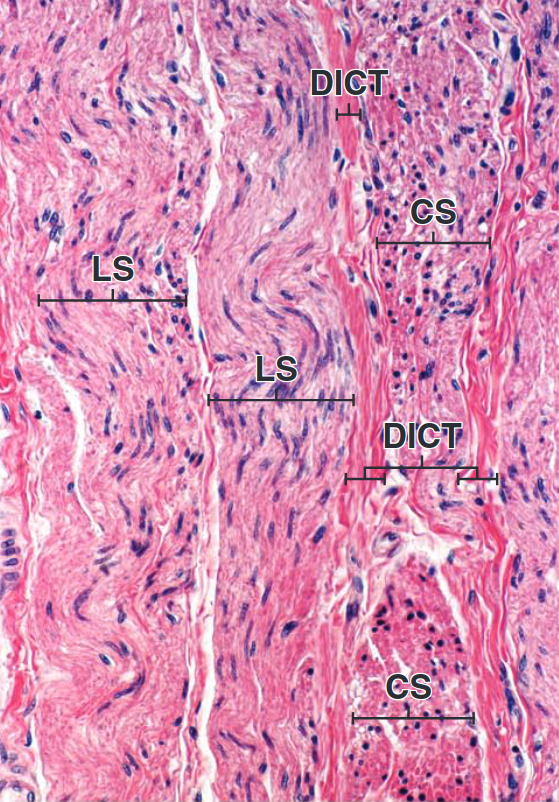
\includegraphics[scale=0.25]{images/week-1-rp11.jpg} 
    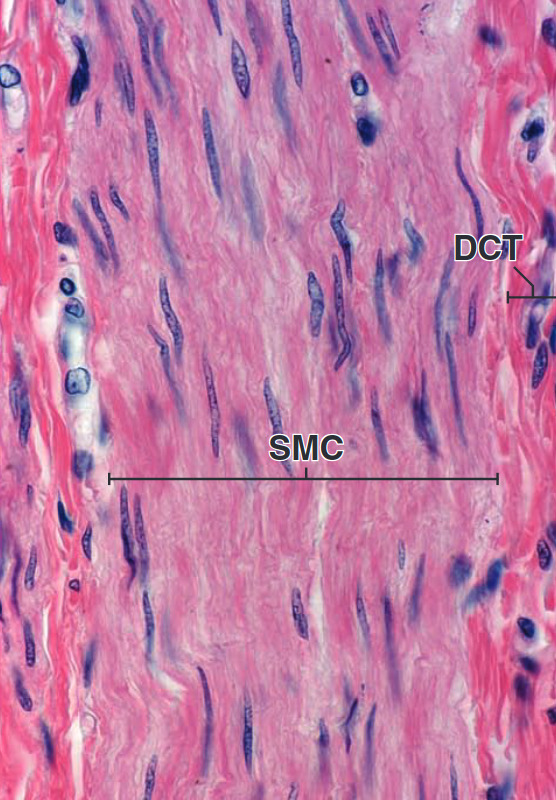
\includegraphics[scale=0.25]{images/week-1-rp12.jpg}

    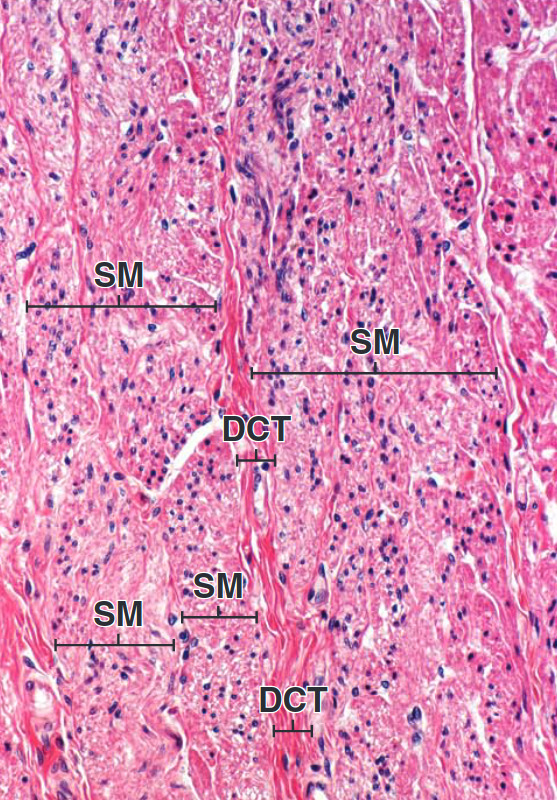
\includegraphics[scale=0.25]{images/week-1-rp13.jpg} 
    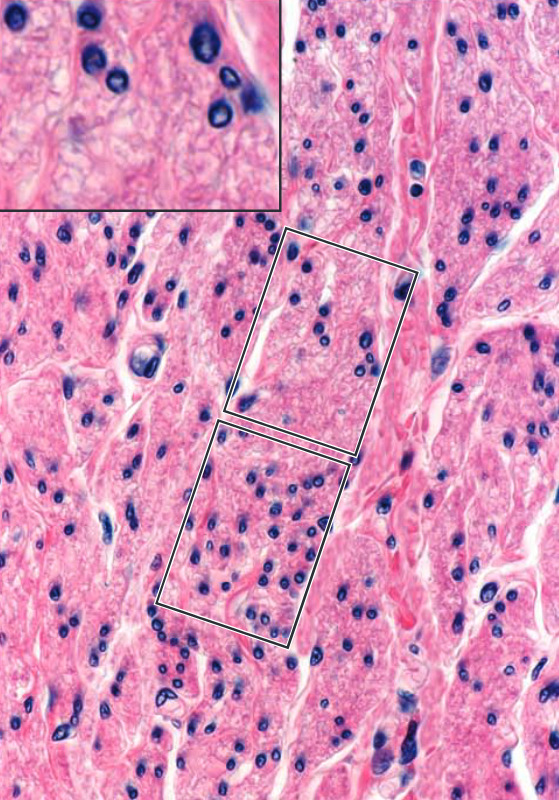
\includegraphics[scale=0.25]{images/week-1-rp14.jpg}
  \end{center}
\end{itemize}